\chapter{控制系统的校正}
\thispagestyle{empty}

\section{系统校正设计基础}
\subsection{性能指标}
\begin{enumerate}[1. ]
	\begin{minipage}{0.5\linewidth}
		\item \textbf{时域指标}\vspace*{-0.5em}
		\begin{itemize}
			\item 超调量 \quad $\sigma \%$\vspace*{-0.5em}
			\item 调节时间 \quad $t_{\text{s}}$\vspace*{-0.5em}
			\item 上升时间 \quad $t_{\tau}$\vspace*{-0.5em}
			\item 无差度 \quad $\nu$\vspace*{-0.5em}
			\item 稳态误差、开环增益等
		\end{itemize}
	\item \textbf{复数域指标}\\
	系统的闭环极点在复平面上的分布区域。\vspace*{-0.5em}
	\begin{itemize}
		\item 振荡度 \quad $\varphi$\vspace*{-0.5em}
		\item 衰减度 \quad $\eta$
	\end{itemize}
	\end{minipage}
	\begin{minipage}{0.7\linewidth}
	\item \textbf{频域指标}\vspace*{-0.5em}
	\begin{itemize}
		\item 闭环频率特性
		\begin{itemize}
			\item 峰值比 \quad $\dfrac{M_{\text{m}}}{M_{\text{o}}}$
			\item 峰值频率 \quad $\omega_{\text{m}}$
			\item 频带宽度 \quad $\omega_{\text{b}}$
		\end{itemize}
		
		\item 开环频率特性
		\begin{itemize}
			\item 截止频率 \quad $\omega_{\text{c}}$
			\item 相稳定裕度 \quad $\gamma$
			\item 模稳定裕度 \quad $h$
		\end{itemize}
	\end{itemize}
	\end{minipage}
\end{enumerate}
	
\begin{figure}[!htb]
	\centering
	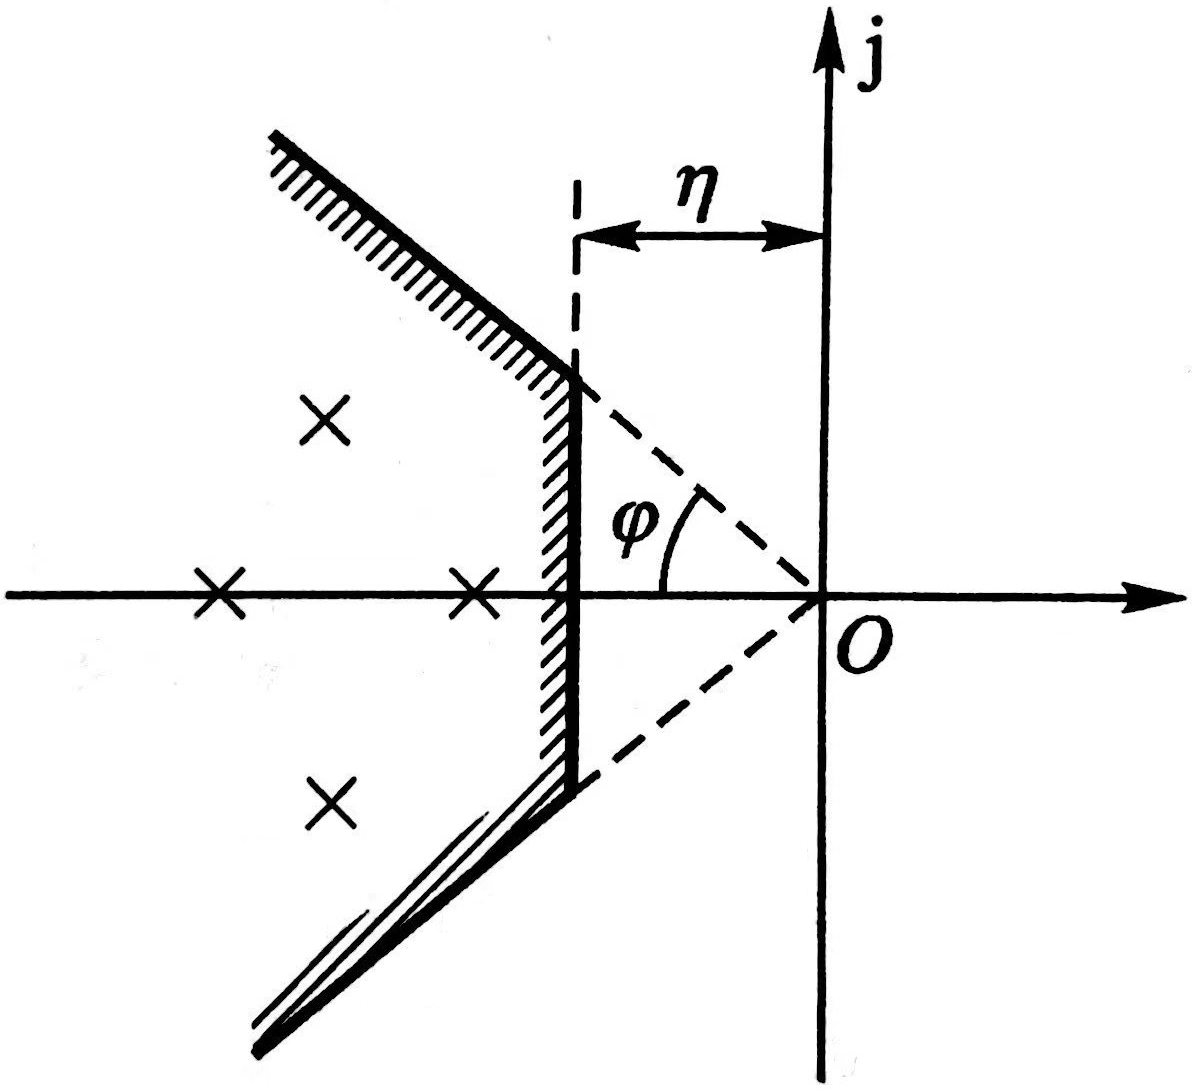
\includegraphics[width=0.3\linewidth]{pic/复数域性能指标.jpeg}
	\vspace*{-1em}
	\caption{闭环极点的限制区域}
	\label{复数域性能指标}
\end{figure}

\subsection{校正方式}
	在系统基本部分已经确定的情况下,为了保证系统满足动态特性指标,往往需要在系统中附加上一些具有一定动力学性质的附加装置,这些附加装置统称为\dy[校正元件]{JZYJ}或\dy[校正装置]{JZZZ}。
	
	常见的校正装置有以下四种:
	
\begin{equation*}
	\mbox{校正方式}\,
	\begin{cases}
		\, \mbox{串联校正}\\
		\, \mbox{反馈校正}\\
		\, \mbox{(前馈)顺馈校正}\,
		\begin{cases}
			\, \mbox{前置校正}\\
			\, \mbox{干扰补偿}
		\end{cases}
	\end{cases}
\end{equation*}

\begin{figure}[!htb]
	\centering
	\begin{tikzpicture}[circuit ee IEC]
			%定义流程图具体形状
		\node(O) [minimum height=0cm,draw, node distance=1cm,inner sep=5pt] {前置校正};
		\node[bulb] (A)[minimum height=0cm,draw,below of = O,xshift = -2cm,node distance=1.5cm,inner sep=5pt, label = -95:$-$] { };
		\node (B) [minimum height=0cm,draw,below of = O, xshift = -0cm,node distance=1.5cm, inner sep=5pt] {控制器};
		\node[bulb] (D) [minimum height=0cm,draw,below of = O, xshift = 2cm,node distance=1.5cm, inner sep=5pt] { };
		\node (C) [draw, right of = D, node distance = 1.5cm, inner sep = 5pt]{对象};
		\node (E) [draw, left of = A, node distance = 2cm, inner sep = 5pt]{前置校正};

		%连接具体形状
		\draw[arrows={-Stealth}](2cm,1cm) -- (D)  node[midway,right = 0.6cm, above=0.5cm]{干扰$N$};
		\draw[arrows={-Stealth}](2cm,1cm) -- (2cm,0) -- (O) ;
		\draw[arrows={-Stealth}](O) --+(-2cm,0) -- (A) ;
		\draw[arrows={-Stealth}](-7cm,-1.5cm) -- (E)  node[midway,above=0cm]{给定值R};
		\draw[arrows={-Stealth}](E) -- (A) ;
		\draw[arrows={-Stealth}](A) -- (B) ;
		\draw[arrows={-Stealth}](B) -- (D) ;
		\draw[arrows={-Stealth}](D) -- (C) ;
		\draw[arrows={-Stealth}](C) -- +(3cm,0) node[midway,above=0cm]{被控量C} ;
		\draw[arrows={-Stealth}](5.2cm,-1.5cm) --+(0,-1.5cm) --+(-7.2cm, -1.5cm) -- (A) ;
	\end{tikzpicture}
	\caption{前置校正}
	\label{前置校正}
\end{figure}
\begin{figure}[!htb]
	\centering
	\begin{tikzpicture}[circuit ee IEC]
		%定义流程图具体形状
		\node[bulb] (A) [inner sep = 5pt, draw, label = -95:$-$]{};
		\node (B) [inner sep = 5pt, right of = A, node distance = 2cm, draw]{串联校正};
		\node[bulb] (C) [inner sep = 5pt, right of = B, node distance = 2cm, draw, label = -95:$-$]{};
		\node (D) [inner sep = 5pt, right of = C, node distance = 2cm, draw]{控制器};
		\node (E) [inner sep = 5pt, right of = D, node distance = 2cm, draw]{对象};
		\node (F) [inner sep = 5pt, below of = E, xshift = -12mm, node distance = 1.2cm, draw]{反馈校正};
		
		%连接具体形状
		\draw[arrows={-Stealth}](-3cm, 0cm) -- (A)  node[midway,above=0cm]{给定值R};
		
		\draw[arrows={-Stealth}](A) -- (B) ;
		\draw[arrows={-Stealth}](B) -- (C) ;
		\draw[arrows={-Stealth}](C) -- (D) ;
		\draw[arrows={-Stealth}](D) -- (E) ;
		\draw[arrows={-Stealth}](E) -- +(3cm,0) node[midway,above=0cm]{被控量C} ;
		\draw[arrows={-Stealth}](9.5cm, 0cm) -- +(0cm, -1.2cm) -- (F) ;
		\draw[arrows={-Stealth}](F) -- (4cm, -1.2cm) -- (C) ;
		\draw[arrows={-Stealth}](9.5cm, -1.2cm) -- +(0cm, -1.2cm) -- (0cm,-2.4cm) -- (A) ;
	\end{tikzpicture}
	\caption{串联校正和反馈校正}
	\label{串联校正和反馈校正}
\end{figure}

\section{串联校正}
加入串联校正后的系统结构图如图\ref{系统的串联校正}所示。其中$G_{\text{c}}(s)$表示了串联校正装置的传递函数,$G(s)$表示系统不变部分的传递函数。
\begin{equation*}
	\mbox{串联校正} \,
	\begin{cases}
		\, \mbox{超前校正}\\
		\, \mbox{滞后校正}\\
		\, \mbox{滞后—超前校正}
	\end{cases}
\end{equation*}
\begin{figure}[!htb]
	\centering
	\begin{tikzpicture}[circuit ee IEC]
		%定义流程图具体形状
		\node[bulb] (A) [inner sep = 5pt, draw, label = -95:$-$]{};
		\node (B) [inner sep = 5pt, right of = A, node distance = 2cm, draw]{$G_{\text{c}}(s)$};
		\node (C) [inner sep = 5pt, right of = B, node distance = 2cm, draw]{$G(s)$};
		
		%连接具体形状
		\draw[arrows={-Stealth}](-1.5cm, 0cm) -- (A);
		
		\draw[arrows={-Stealth}](A) -- (B) ;
		\draw[arrows={-Stealth}](B) -- (C) ;
		\draw[arrows={-Stealth}](C) -- +(2cm,0) ;
		\draw[arrows={-Stealth}](5.2cm , 0cm) -- (5.2cm, -1.2cm) -- (0cm,-1.2cm) -- (A) ;
	\end{tikzpicture}
	\vspace*{-0.5em}
	\caption{系统的串联校正}
	\label{系统的串联校正}
\end{figure}
\vspace*{-0.5em}

\subsection{相位超前校正}\vspace*{-0.5em}\index{CQJZ@超前校正}
\begin{enumerate}[1. ]
	\item \textbf{相位超前校正的特点}\vspace*{-0.5em}
	\begin{itemize}
		\item 超前补偿可显著改善系统的动态品质而对系统稳态性能影响较小;
		\item 但经超前补偿后的系统高频噪声的抑制能力会下降。
	\end{itemize}

	\item \textbf{超前补偿器的数学模型}
	\begin{align}
		G_{\text{c}}(s) &= K_c \dfrac{aTs + 1}{Ts + 1},\quad \quad a>1\\
		\varPhi(\omega) = \angle G_{\text{c}}(\j \omega) &= \arctan aT\omega - \arctan T\omega
	\end{align}

\begin{figure}[!htb]
	\centering
	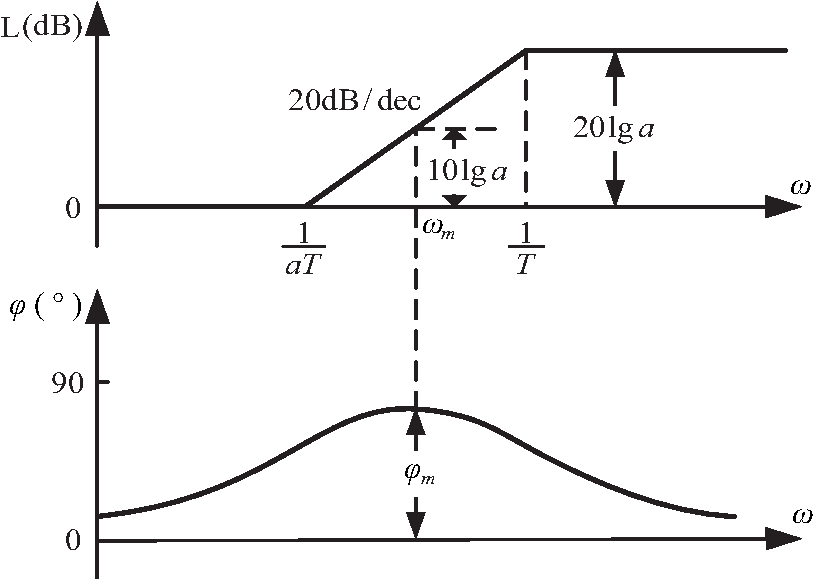
\includegraphics[width=0.55\linewidth]{pic/超前bode.pdf}
	\vspace*{-1em}
	\caption{超前校正的Bode图}
	\label{超前Bode}
\end{figure}
其中,
\begin{align}
	\omega_\text{m} &= \dfrac{1}{T \sqrt{a}}\\
	\varphi_\text{m} &= \arcsin \dfrac{a - 1}{a + 1}
\end{align}

	\item \textbf{超前补偿器的设计步骤}\\
	设系统原传递函数为$G_1(s)$,补偿器的传递函数为$G_\text{c}(s)$.\vspace*{-0.5em}
	\begin{enumerate}[\textbf{步骤} 1 ]
		\item \textbf{确定需要增加的相角}$\varphi_{\text{m}}$
		\begin{equation}
			\varphi_{\text{m}} = \gamma' - \gamma +(5\degree \sim 12 \degree)
		\end{equation}
		其中,$\gamma'$指的是期望的相稳定裕度。
		
		\item \textbf{确定参数$a$}
		\begin{align}
			a = \dfrac{1 + \sin \varphi_\text{m}}{1 - \sin \varphi_\text{m}}
		\end{align}
		
		\item \textbf{确定新的截止频率$\omega_{\text{c}}'$}
		\begin{equation}
			20 \lg A(\omega_{\text{c}}') = - 10 \lg a
		\end{equation}
		
		\item \textbf{确定新的转折频率对应的$T$}
		\begin{align}
			\omega_{\text{c}}' = \omega_{\text{m}} = \dfrac{1}{T \sqrt{a}} \quad \Rightarrow \quad T = \dfrac{1}{\omega_{\text{c}}'\sqrt{a}}
		\end{align}
	\end{enumerate}
若已知$\omega_{\text{c}}' \ge \omega^*$,则步骤可以简化为
\begin{enumerate}[\textbf{步骤}]
	\item $2^*\,\,$ \textbf{确定新的截止频率$\omega_{\text{c}}'$}
	\begin{equation}
		\omega_{\text{c}}' = \omega^* + (3 \sim 5)
	\end{equation}
	
	\item $3^*\,\,$ \textbf{确定补偿器的参数和转折频率}
	\begin{equation}
		10 \lg a = - 20 \lg|G(\j \omega_{\text{c}}')| \quad \Rightarrow \quad a \quad \Rightarrow \quad \dfrac{1}{T} = \sqrt{a}\omega_{\text{c}}
	\end{equation}
\end{enumerate}
\end{enumerate}
\clearpage

\vspace*{-3em}
\examples \label{6.1}考虑如下系统,其开环传递函数用$G(s)$表示
\begin{figure}[!htb]
	\centering
	\begin{tikzpicture}[circuit ee IEC,node distance=1.2cm]
		\node[bulb] (A)  [draw, inner sep=5pt,label=-80:$-$] {};
		\node (B) [draw, inner sep =4pt,right of = A, node distance = 2cm]{$\,\dfrac{K}{s(0.1s + 1)}\,$};
		
		\draw[arrows={-Stealth}] (-1cm,0cm) -- (A)node[near start, above = 0cm]{$R(s)$};
		\draw [arrows={-Stealth}] (A) -- (B);
		\draw[arrows={-Stealth}] (B) -- (4cm,0cm)node[near end, above =0cm]{$C(s)$};
		\draw[arrows={-Stealth}] (3.5cm,0cm) -- +(0cm, -1cm) -- (0cm,-1cm) -- (A);
	\end{tikzpicture}
	\caption{\ref{6.1} 系统结构图}
	\label{F6.1.1}
\end{figure}

要求设计一个串联补偿器,使得静态速度误差$e_{\text{ss}} \le 0.01, \gamma \ge 45\degree, \omega_{\text{c}} \ge 40$rad/s.

\solve 根据上面的步骤解题。
\begin{enumerate}[\textbf{第} 1 \textbf{步} ]
	\item \textbf{确定满足稳态误差的开环增益$K$}\\
	由于这是一个\RMN[1]型系统,所以$e_{\text{ss}} = \dfrac{1}{K} \le 0.01 \quad \Rightarrow \quad K \ge 100$.不妨取$K = 100.$
	
	\item \textbf{求此时的相稳定裕度}\\
	经过计算,绘制Bode图如图\ref{F6.1.2}.
	\begin{figure}[!htb]
		\centering
		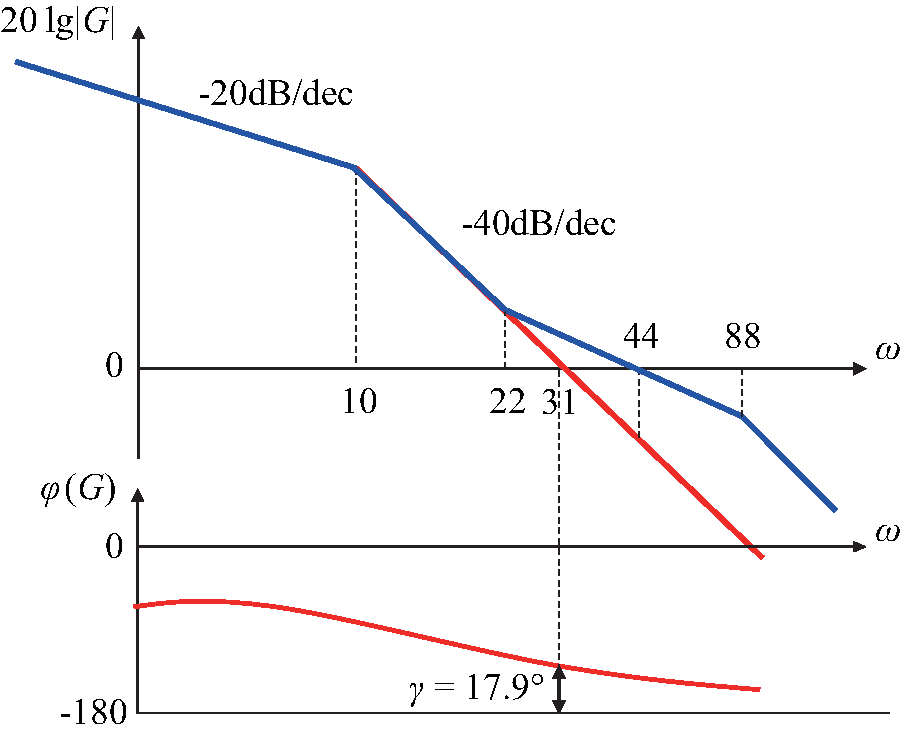
\includegraphics[width=0.45\linewidth]{pic/6.1.pdf}
		\vspace*{-1em}
		\caption{\ref{6.1}修正前的Bode图}
		\label{F6.1.2}
	\end{figure}

	从而得到
	\begin{align*}
		\omega_{\text{c}} &= 31 \text{rad/s}\\
		\gamma &= 17.9 \degree
	\end{align*}
	
	\item \textbf{确定新的截止频率}\\
	由于要求$\omega_{\text{c}} \ge 40$rad/s,不妨选取
	\[
	\omega_{\text{c}}' = \omega_{\text{m}} = 44 \text{rad/s}
	\]
	
	\item \textbf{计算未经校正系统的幅值}
	\[
	20 \lg |G(\j \omega_{\text{c}}')| = -6 \text{dB} 
	\]
	
	\item \textbf{确定补偿器的参数和转折频率}
	\[
	10 \lg a = 6 \text{dB} \quad \Rightarrow \quad a = 4 \quad \Rightarrow \quad \dfrac{1}{T} = \sqrt{a}\omega_{\text{c}} = 88
	\]
\end{enumerate}
所以
\[
\dfrac{G_\text{c}(s)}{K_\text{c}} = \dfrac{aTs + 1}{Ts + 1} = \dfrac{0.04544s + 1}{0.01136s + 1}
\]
用Matlab绘制补偿前后系统的Bode图如图\ref{F6.1.3}.
\begin{figure}[!htb]
	\centering
	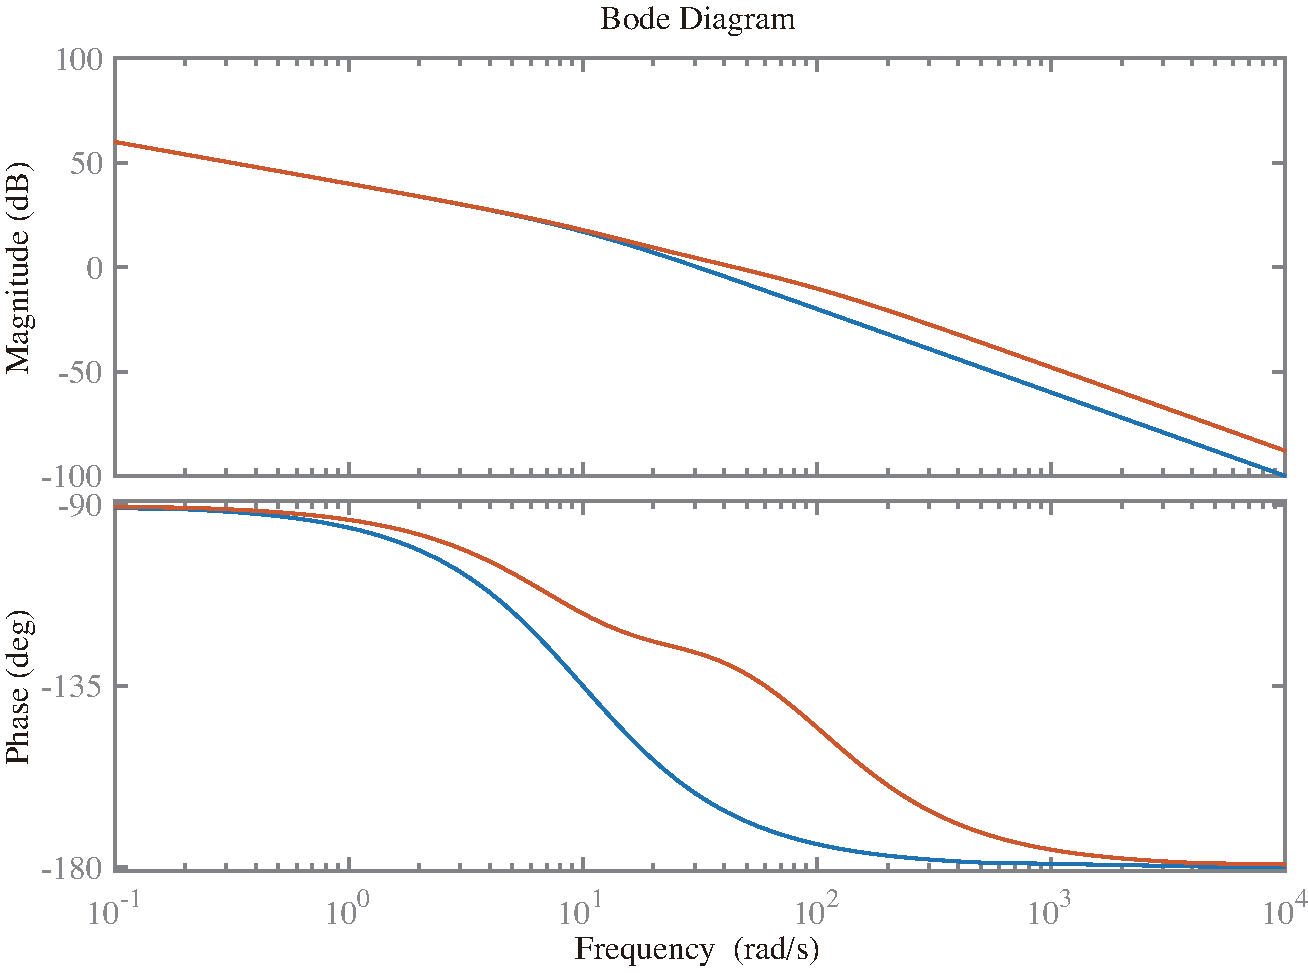
\includegraphics[width=0.6\linewidth]{pic/6.1.2.pdf}
	\vspace*{-1em}
	\caption{\ref{6.1}修正前后的Bode图}
	\label{F6.1.3}
\end{figure}

\subsection{相位滞后校正}\vspace*{-0.5em}\index{ZHJZ@滞后校正}
\begin{enumerate}[1. ]
	\item \textbf{相位滞后校正的特点}\\
	(1) 滞后校正的主要功能是抑制高频干扰并使经校正后的系统具有较大的相稳定裕度。\\
	(2) 滞后补偿器本质上是一个低通滤波器,因此,滞后 校正可允许低频段有高增益。\\
	(3) 离虚轴很近的极点会对系统的过渡过程产生影响, 使响应变慢(尽管其附近的零点可使幅值变小)。\\
	(4) 截止频率$\omega_{\text{c}}' < \omega_{\text{c}}$,从而使调节时间$t_\text{s}$增加。
	
	\item \textbf{滞后补偿器的数学模型}
	\begin{align}
		G_{\text{c}}(s) &= K_c \dfrac{bTs + 1}{Ts + 1}, \quad \quad 0 < b < 1\\
		\varPhi(\omega) = \angle G_{\text{c}}(\j \omega) &= \arctan bT\omega - \arctan T\omega
	\end{align}
	
	\begin{figure}[!htb]
		\centering
		\includegraphics[width=0.55\linewidth]{pic/滞后bode.pdf}
		\vspace*{-1em}
		\caption{滞后校正的Bode图}
		\label{滞后Bode}
	\end{figure}
	其中,
	\begin{align}
		\omega_\text{m} &= \dfrac{1}{T \sqrt{b}}\\
		\varphi_\text{m} &= \arcsin \dfrac{1 - b}{1 + b}
	\end{align}
	
	\item \textbf{滞后补偿器的设计步骤}\\
	设系统原传递函数为$G_1(s)$,补偿器的传递函数为$G_\text{c}(s)$.\vspace*{-0.5em}
	\begin{enumerate}[\textbf{步骤} 1 ]
		\item \textbf{根据给定的$\gamma^*$确定$\omega_{\text{c}}'$}
		\begin{equation}
			\gamma' = \gamma^* + (5\degree \sim 12 \degree)
		\end{equation}
		然后根据渐近幅频特性曲线和Bode图计算$\omega_{\text{c}}'$。
		
		\item \textbf{确定参数$b$}
		\begin{align}
			20 \lg b = -20 \lg |G_1(\j \omega_{\text{c}}')| \quad \Rightarrow \quad b = \dfrac{1}{G_1(\j \omega_{\text{c}}')}
		\end{align}
		
		\item \textbf{确定新的转折频率$\dfrac{1}{bT},\dfrac{1}{T}$}
		\begin{align}
			\dfrac{1}{bT} = (0.1 \sim 0.5)\omega_{\text{c}}'
		\end{align}
	\end{enumerate}
\end{enumerate}

\examples \label{6.2}已知单位负反馈系统的开环传递函数为
\[
G(s) = \dfrac{1}{s(0.5s + 1)}
\]
要求在单位斜坡输入下的稳态误差为0.05且相稳定裕度至少45$\degree$,设计串联校正补偿器。

\solve 根据上面的步骤解题。
\begin{enumerate}[\textbf{第} 1 \textbf{步} ]
	\item \textbf{确定满足稳态误差的开环增益$K$}\\
	$G_1(s) = K \dfrac{1}{s(0.5s + 1)}$,由于这是一个\RMN[1]型系统,所以$e_{\text{ss}} = \dfrac{1}{K} = 0.05 \quad \Rightarrow \quad K = 20$.
	
	\item \textbf{求此时的相稳定裕度}\\
	经过计算,绘制Bode图如图\ref{F6.2.1}.
	\begin{figure}[!htb]
		\centering
		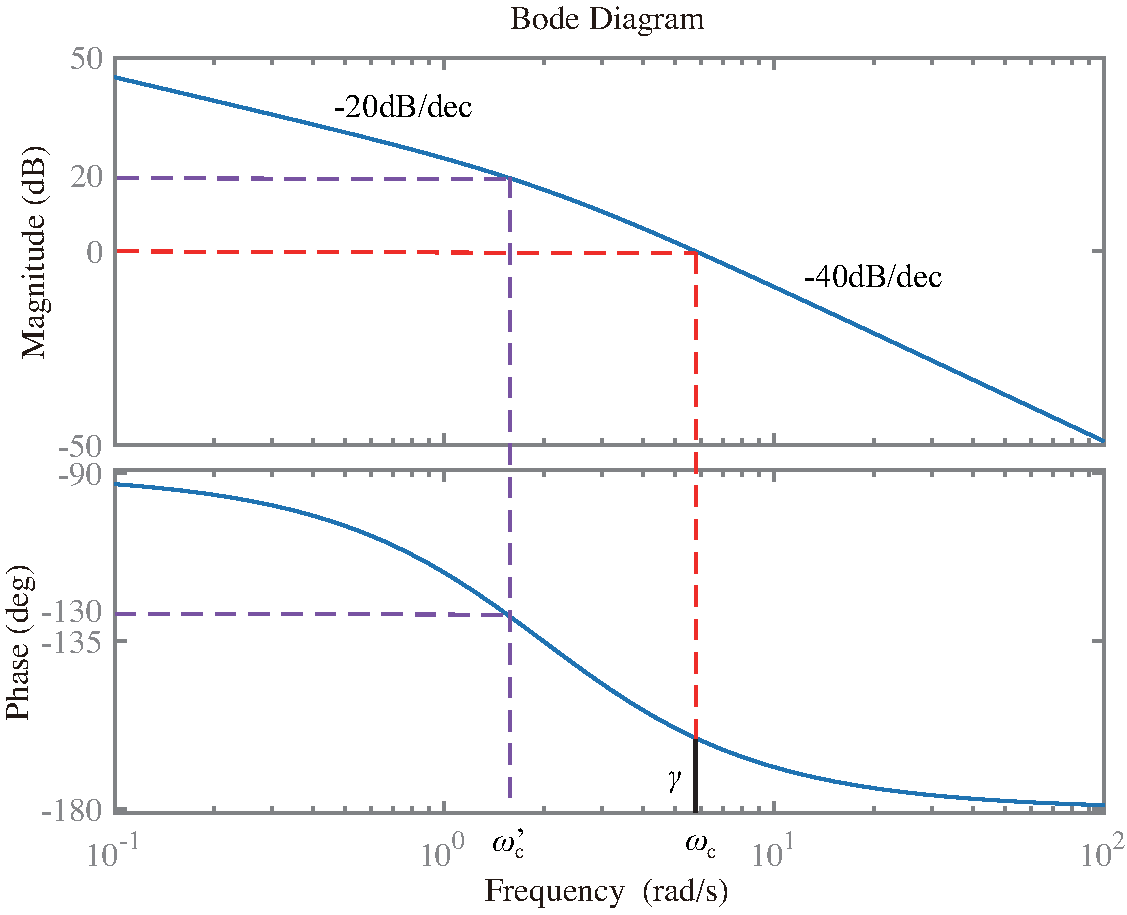
\includegraphics[width=0.7\linewidth]{pic/6.2.1.pdf}
		\vspace*{-1em}
		\caption{\ref{6.2}修正前的Bode图}
		\label{F6.2.1}
	\end{figure}
	
	可以用渐近幅频特性曲线计算截止频率和对应的相温度裕度
	\begin{align*}
		L(\omega) = 20\lg K - 20\lg \omega - 20 \lg T_1\omega = 20\lg 20 - 20\lg \omega &- 20 \lg 0.5\omega = 0 \quad \Rightarrow \quad \omega_{\text{c}} = 2\sqrt{10} \approx 6.3 \,\,\text{rad/s}\\
		\varphi(\omega_{\text{c}}) = -90\degree - \arctan(0.5 \omega_{\text{c}}) &= -162\degree \quad \Rightarrow \quad \gamma = 18\degree
	\end{align*}
	
	\item \textbf{确定新的截止频率}\\
	取$\gamma' = 50 \degree$($5\degree$用于补偿相位滞后),得
	\[
	\varphi(\omega_{\text{c}}) = -130 \degree \quad \Rightarrow \quad \omega_{\text{c}}' = 1.5 \,\,\text{rad/s}
	\]
	
	\item \textbf{计算未经校正系统的幅值}
	\[
	20 \lg |G(\j \omega_{\text{c}}')| = 20 \text{dB} 
	\]
	
	\item \textbf{确定补偿器的参数和转折频率}
	\[
	20 \lg b = -20 \text{dB} \quad \Rightarrow \quad b = 0.1 
	\]
	选择
	\[
	\dfrac{1}{bT} = 0.1 \omega_{\text{c}}' = 0.15 \quad \Rightarrow \quad \dfrac{1}{T} = 0.015
	\]
	
\end{enumerate}
\begin{figure}[!htb]
	\centering
	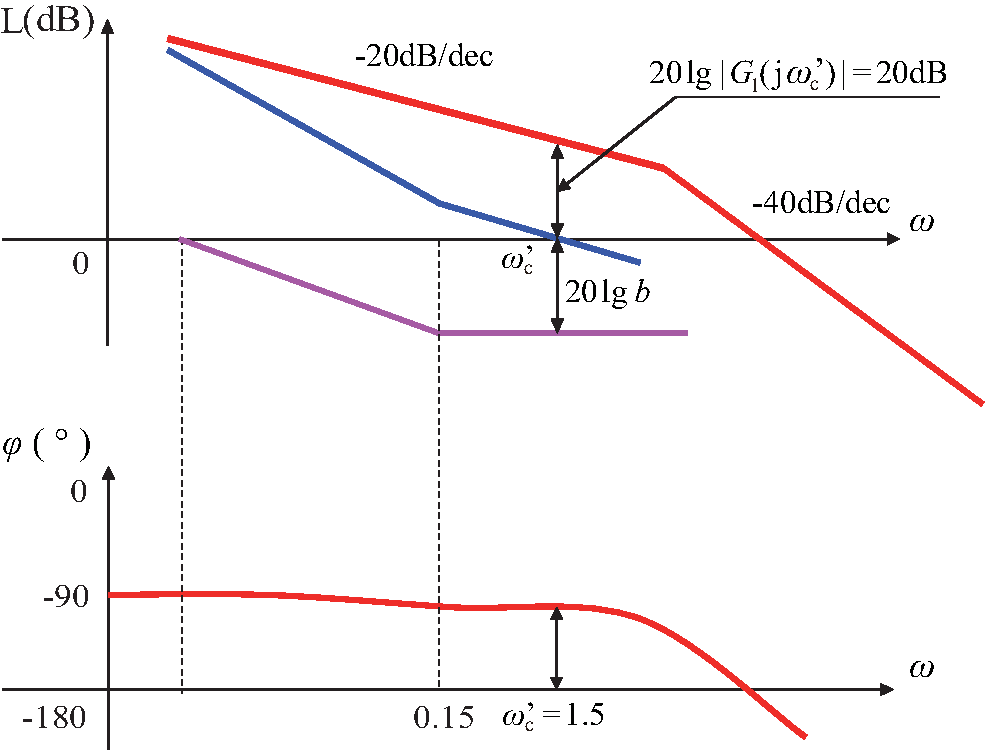
\includegraphics[width=0.6\linewidth]{pic/6.2.2.pdf}
	\vspace*{-1em}
	\caption{\ref{6.2}确定新的截止频率}
	\label{F6.2.2}
\end{figure}
所以设计的补偿器为
\[
\dfrac{G_\text{c}(s)}{K_\text{c}} =  \dfrac{bTs + 1}{Ts + 1} = \dfrac{6.67s + 1}{66.7s + 1}
\]
用Matlab绘制补偿前后系统的Bode图如图\ref{F6.2.3}.
\begin{figure}[!htb]
	\centering
	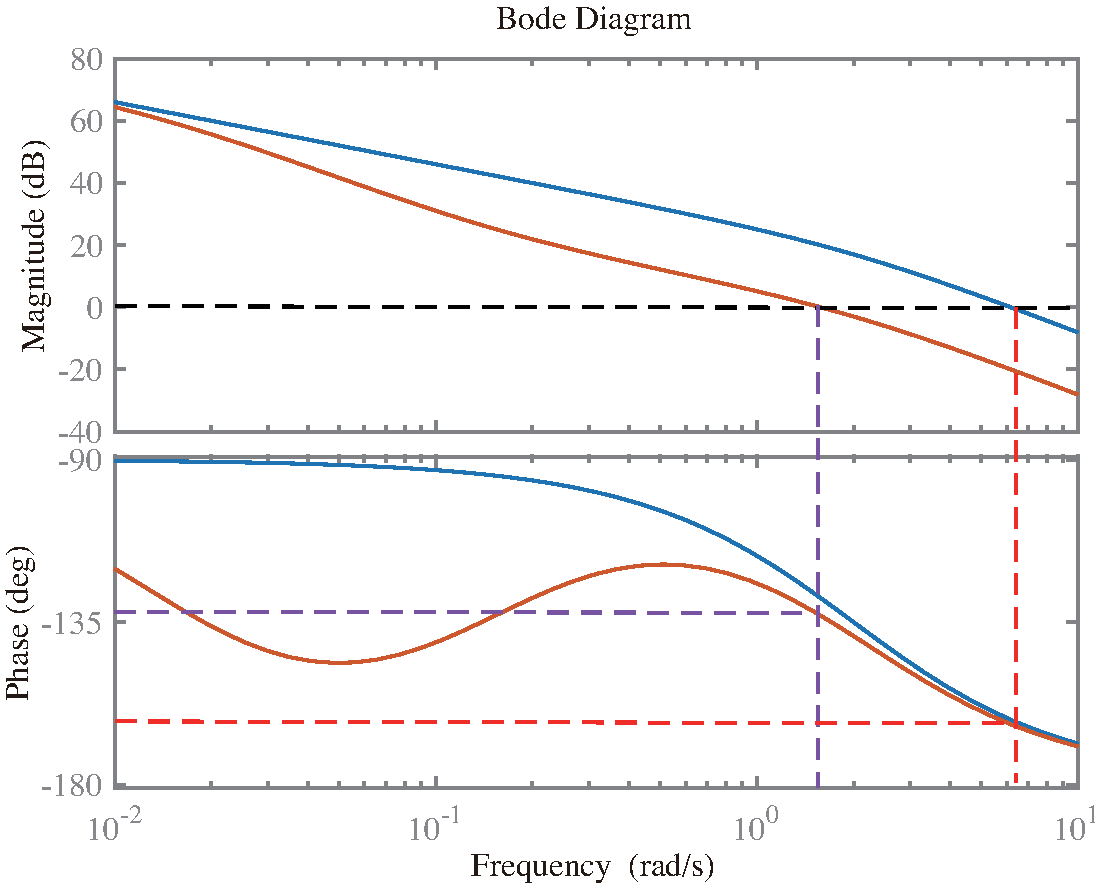
\includegraphics[width=0.6\linewidth]{pic/6.2.3.pdf}
	\vspace*{-1em}
	\caption{\ref{6.2}修正前后的Bode图}
	\label{F6.2.3}
\end{figure}

\subsection{超前—滞后校正}\vspace*{-0.5em}\index{CQZHJZ@超前—滞后校正}
\begin{enumerate}[1. ]
	\item \textbf{相位滞后校正的特点}\\
	(1) 超前校正可改善响应速度和相稳定裕度,但会导致频宽增加,不利于高频干扰的抑制。\\
	(2) 滞后校正可改善相稳定裕度,但有会使调节时间变长。\\
	(3) 因此,希望用滞后—超前校正将以上两种校正器的优点结合在一起。
	
	\item \textbf{滞后补偿器的数学模型}
	\begin{align}
		G_{\text{c}}(s) &= K_c\left(\dfrac{bT_1s + 1}{T_1s + 1}\right) \left(\dfrac{aT_2s + 1}{T_2s + 1}\right), \quad \quad a>1, \, 0 < b < 1, \, bT_1 > aT_2\\
		\varPhi(\omega) &= \angle G_{\text{c}}(\j \omega) = \arctan bT\omega - \arctan T\omega
	\end{align}
	通常要求滞后部分的两个转折频率要低于超前部分的两个转折频率。
	
	\begin{figure}[!htb]
		\centering
		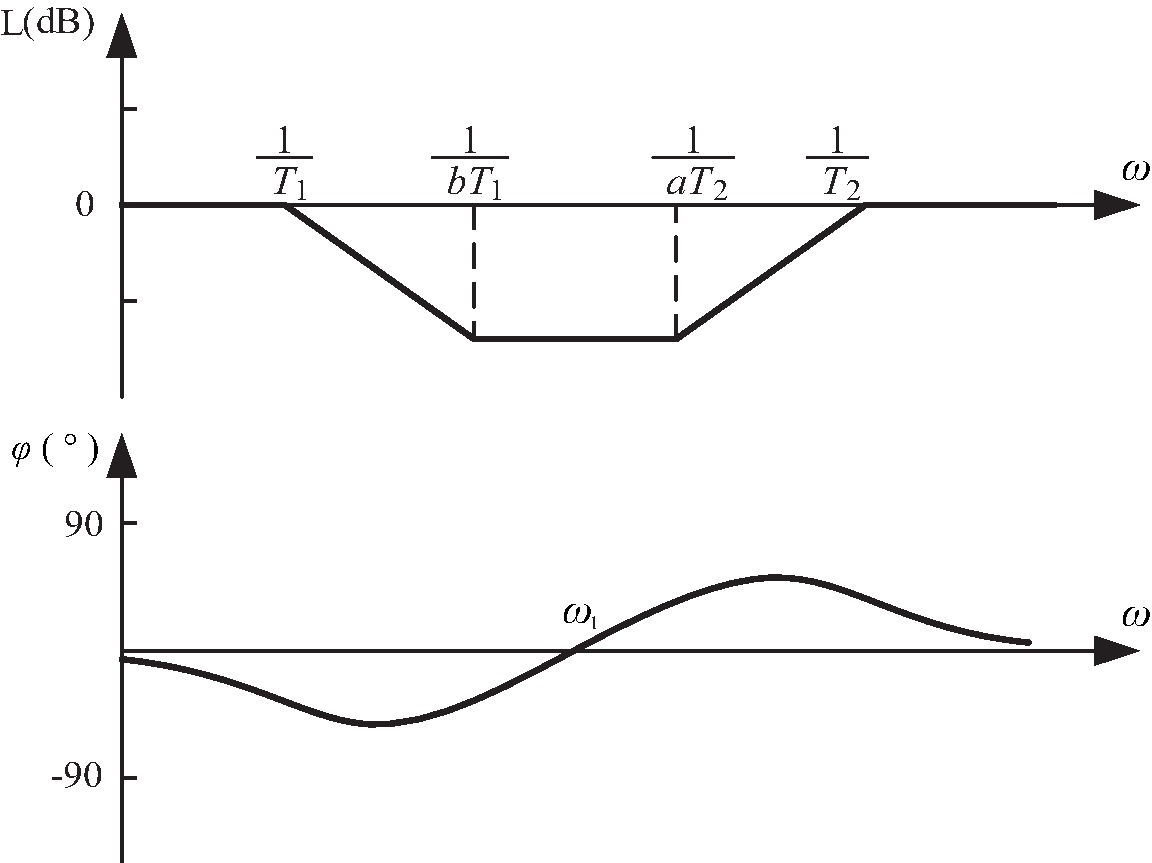
\includegraphics[width=0.55\linewidth]{pic/超前滞后Bode图.pdf}
		\vspace*{-1em}
		\caption{超前—滞后校正的Bode图}
		\label{超前滞后Bode}
	\end{figure}
\end{enumerate}

\vspace*{-2.5em}

\warn[
\textbf{\large 频率校正总结}\\
\hspace*{1em} 三种校正方法均基于镜像原理,一般地:
\vspace*{-0.5em}
{
	\begin{enumerate}[\hspace*{2em} 1. ]
		\item 根据相稳定裕度确定校正后的截止频率$\omega_{\text{c}}'$
		\vspace*{-0.5em}
		
		\item 利用镜像原理求校正器的交接频率,即新的截止频率$\omega_{\text{c}}'$处补偿器的幅值和被补偿系统的幅值互补,相加为0.
	\end{enumerate}
}
]

\subsection{PID校正器}
\begin{enumerate}
	\item \textbf{PD校正器}\\
	\dy[PD校正器]{PDJZQ}又称为\dy[比例—微分校正]{BLWFJZ},其传递函数
	\begin{align}
		G_{\text{c}}(s) & = K_{\text{d}} s + K_{\text{p}}\\
		& = K_{\text{p}}\left(\dfrac{K_{\text{d}}}{K_{\text{p}}}s + 1\right) = K_{\text{p}}(Ts + 1)
	\end{align}
	其作用相当于超前校正。
	
	\item \textbf{PI校正器}\\
	\dy[PI校正器]{PIJZQ}又称为\dy[比例—积分校正]{BLJFJZ},其传递函数
	\begin{align}
		G_{\text{c}}(s) = K_{\text{p}}  + \dfrac{1}{T_{\text{i}} s} = \dfrac{1}{T_{\text{i}}} \dfrac{T_{\text{i}} K_{\text{p}}s + 1}{s}
	\end{align}
	其作用相当于滞后校正。
	
	\item \textbf{PID校正器}\\
	\dy[PID校正器]{PIDJZQ}又称为\dy[比例—积分—微分校正]{BLJFWFJZ},其传递函数
	\begin{align}
		G_{\text{c}}(s) = K_{\text{p}}  + K_\text{d} s +  \dfrac{1}{T_{\text{i}} s} = \dfrac{T_\text{i} K_{\text{d}}s^2 + T_\text{i} K_\text{p}s + 1}{T_{\text{i}}s}
	\end{align}
	其作用相当于超前—滞后校正。

\end{enumerate}


\section{串联校正的根轨迹方法}
\subsection{增加零、极点对系统性能的影响}
\noindent \textbf{1. 增加极点对系统性能的影响}


在开环传递函数中增加一个极点会使根轨迹向虚轴偏移,降低相对稳定性及延长调节时间。


\noindent \textbf{2. 增加零点对系统性能的影响}


在开环传递函数中增加一个零点会使根轨迹向左偏移,使系统更加稳定且响应速度更快。

\subsection{根轨迹校正器设计}

\noindent \textbf{1. 数学模型}
\begin{equation}
	G_{\text{c}}(s) = K_\text{c} \dfrac{aTs+1}{Ts + 1} = K_\text{c}^* \dfrac{s + \dfrac{1}{aT}}{s + \dfrac{1}{T}} = K_\text{c}^* \dfrac{s - z}{s - p}, \quad a>1
\end{equation}

\noindent \textbf{2. 设计步骤}
\begin{enumerate}[\hspace*{2em} \textbf{步骤} 1 ]
	\item \textbf{由二阶系统的性能指标确定主导极点}
	\begin{equation}
		s_{1,2} = \zeta \omega_{\n} \pm \j \sqrt{1 - \zeta^2} \omega_{\n}
	\end{equation}
	\item \textbf{绘原系统的闭环根轨迹,确定是否仅调节系统的开环增益$\bm{K^*}$就可以达到期望的闭环极点}
	\item \textbf{确定校正器的类型}
	\item \textbf{确定补偿器零点和极点的位置}\\
	通常有无数种取法,工程上一般这么做\vspace*{-0.5em}
	\begin{enumerate}[\hspace*{1em}1.]
		\item 确定满足$\pm180\degree(2k+1)$条件时,需要增加的相角$\varphi$
		\item 利用角平分线补偿相角以确定补偿器零点和极点的位置,如图\ref{根轨迹超前}.
		\begin{enumerate}[(1)  ]
			\item 作水平线$PA$及直线$PO$
			\item 作$\angle APO$的角平分线$PB$
			\item 过$P$点作两条直线$PC,PD$ ,使得与$PB$的角度为$\dfrac{\varphi}{2}$.$PC$和$PD$与横轴的交点就是补偿器极点和零点的位置
			\item 利用角度关系解三角形确定零点$z$和极点$p$的值
		\end{enumerate}
	\end{enumerate}
	\begin{figure}[!htb]
		\centering
		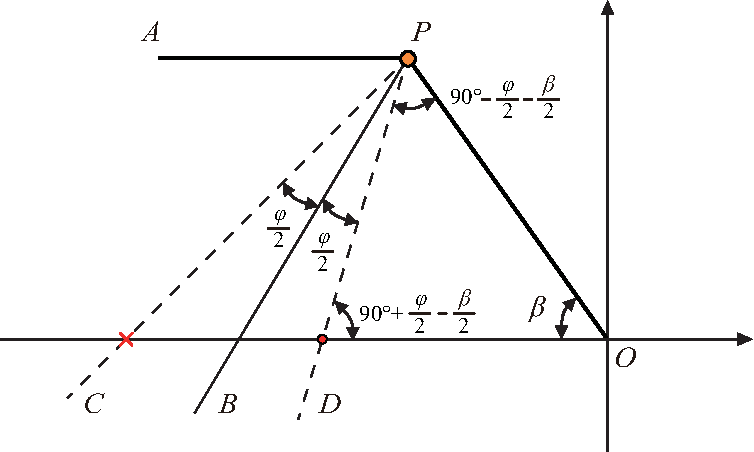
\includegraphics[width=0.55\linewidth]{pic/根轨迹超前.pdf}
		\vspace*{-1em}
		\caption{利用角平分线补偿相角以确定补偿器零点和极点示意图}
		\label{根轨迹超前}
	\end{figure}
	\item \textbf{确定补偿器开环增益$\bm{K_\text{c}^*}$的值}\\
	利用在主导极点处的模方程$\big|G'(s_1)\big|=\Big|G'\left(\zeta \omega_{\n} + \j \sqrt{1 - \zeta^2} \omega_{\n}\right)\Big| = 1$确定开环增益$K_\text{c}^*$的值。
\end{enumerate}

\examples \label{6.4}已知单位负反馈系统的开环传递函数为
\begin{equation}
	G(s) = \dfrac{4}{s(s+2)}
\end{equation}
设计校正装置,使得$t_\text{s} = 1.75 \, \text{s},\,\, \sigma \% = 16.3\%.$

\solve 由上述方法解题
\begin{enumerate}[\textbf{第} 1 \textbf{步}]
	\item \textbf{由性能指标确定主导极点}\\
	由
	\[
	\sigma \% = \e^{-\frac{\pi \zeta}{\sqrt{1 - \zeta^2}}} \times 100\% = 16.3\%, \, t_\text{s} = \dfrac{3.5}{\zeta \omega_{\n}} = 1.75 \quad \Rightarrow \quad \zeta = 0.5\,(\beta = 60 \degree),\,\, \omega_{\n} = 4 \,\text{rad/s}
	\]
	得到期望的闭环主导极点为
	\[
	s_{1,2} = \zeta \omega_{\n} \pm \j\sqrt{1 - \zeta^2}\omega_{\n} = -2 \pm  \j2\sqrt{3}
	\]
	
	\item \textbf{绘制校正前系统的闭环根轨迹}
	\begin{figure}[!htb]
		\centering
		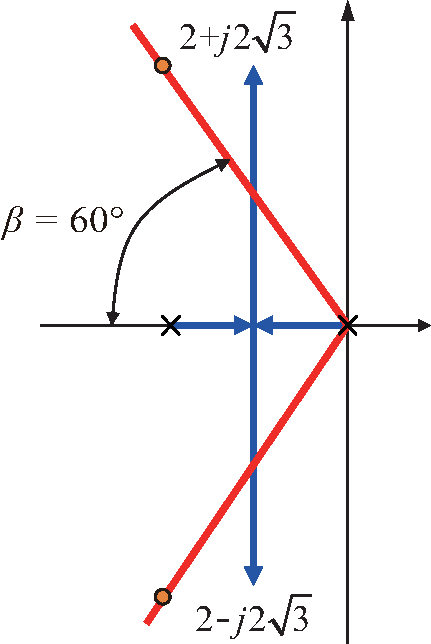
\includegraphics[width=0.25\linewidth]{pic/6.4.1.pdf}
		\caption{\ref{6.4}$\,$校正前系统根轨迹图}
	\end{figure}
	
	\item \textbf{确定校正器的类型}\\
	由根轨迹图可以看出,期望的主导极点在校正前系统的远离虚轴侧,因此,适合采用超前校正器来改变系统的主导极点。设补偿器为
	\[
	G_\text{c}(s) = K_\text{c}\dfrac{s - z}{s -p}, z>p
	\]
	校正后的系统可以表示为
	\[
	G'(s) = G(s)G_\text{c}(s) = \dfrac{4}{s(s+2)}\cdot K_\text{c}\dfrac{s-z}{s-p}
	\]
	
	\item \textbf{确定补偿器零点和极点的位置}
	\begin{enumerate}[1.]
		\item 确定补偿器的相角$\varphi$,校正后的系统在主导极点$s_1 = -2 + \j 2 \sqrt{3}$处满足相角方程
		\[
		\angle G'(s) = \angle G(s) + \angle G_\text{c}(s) = \angle \dfrac{4}{s(s+2)}\Bigg|_{s = 2 + \j 2 \sqrt{3}} + \varphi = 180\degree(2k + 1)
		\]
		计算得到
		\[
			\varphi = 180\degree -  \angle \dfrac{4}{s(s+2)}\Bigg|_{s = 2 + \j 2 \sqrt{3}} = 180 \degree - 150\degree = 30 \degree
		\]
		
		\item 利用角平分线等分法确定零点和极点的位置
		\begin{figure}[!htb]
			\centering
			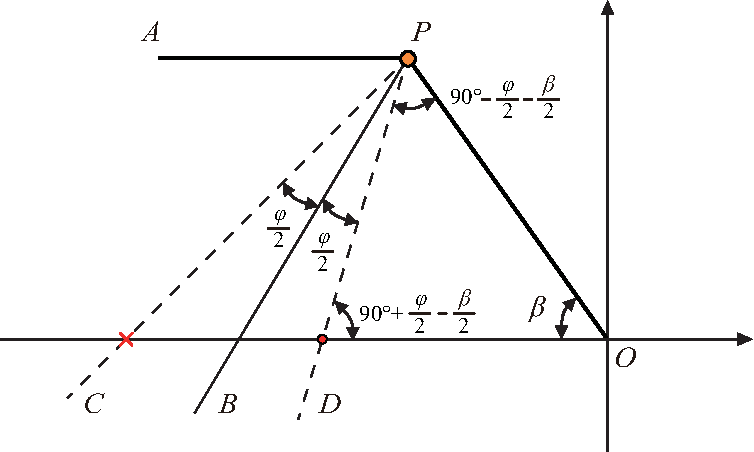
\includegraphics[width=0.55\linewidth]{pic/根轨迹超前.pdf}
			\vspace*{-1em}
			\caption{\ref{6.4}$\,$确定补偿器零点和极点图}
			\label{F6.4}
		\end{figure}
	
		由正弦定理,
		\[
		 |OD| = \dfrac{|OP|}{\sin \left(90 \degree + \dfrac{\varphi}{2} - \dfrac{\beta}{2} \right)} \cdot \sin \left(90 \degree - \dfrac{\varphi}{2} - \dfrac{\beta}{2}\right) = \dfrac{|-2+\j 2 \sqrt{3}|}{\sin (90\degree + 15\degree - 30\degree)}\cdot \sin (90\degree - 15\degree - 30 \degree)=2.93
		\]
		所以,$z = -2.93$,同理可以得到$p = -5.46.$所以校正器和校正后的系统方程分别为
		\begin{align*}
			G_\text{c} (s) &=K_\text{c}^* \dfrac{s + 2.93}{s + 5.46}\\[0.5em]
			G'(s) &= K_\text{c}^* \dfrac{4(s + 2.93)}{s(s+2)(s+5.46)} = K^*\dfrac{s + 2.93}{s(s+2)(s+5.46)} \quad (K^* = 4K_\text{c}^*)
		\end{align*}
	
	\end{enumerate}
	
		\item \textbf{确定补偿器开环增益$\bm{K_\text{c}^*}$的值}\\
		由模方程,得
		\[
			\left|K^* \dfrac{4(s + 2.93)}{s(s+2)(s+5.46)}\right|_{s = -2 + \j 2\sqrt{3}} = 1 \quad \Rightarrow \quad K^* = 18.7 \quad \Rightarrow \quad K_\text{c}^* = K^*/4 = 4.68
		\]
\end{enumerate}
所以校正器和校正后的系统方程分别为
\begin{align*}
	G_\text{c} (s) &=4.68 \dfrac{s + 2.93}{s + 5.46}\\[0.5em]
	G'(s) &= 18.7 \dfrac{4(s + 2.93)}{s(s+2)(s+5.46)}
\end{align*}

\subsection{根轨迹的滞后校正}
若系统具有满意的动态性能但稳态性能不佳,则可考虑采用滞后校正器。即系统有两个主导极点且具有满意的动态响应,但静态速度误差不满足要求。\\[0.5em]
\textbf{根轨迹滞后校正的基本要求}
\begin{itemize}
	\item 不显著改变原闭环主导极点的位置
	\item 开环增益需要调高到满足稳态误差
\end{itemize}

\noindent \textbf{1. 数学模型}
\begin{equation}
	G_{\text{c}}(s) = K_\text{c} \dfrac{bTs+1}{Ts + 1} = K_\text{c}^* \dfrac{s + \dfrac{1}{bT}}{s + \dfrac{1}{T}} = K_\text{c}^* \dfrac{s - z}{s - p}, \quad 0<b<1
\end{equation}

\noindent \textbf{2. 设计步骤}
\begin{enumerate}[\hspace*{2em} \textbf{步骤} 1 ]
	\item \textbf{绘制原系统的根轨迹,并根据动态性能指标确定期望的闭环主导极点在复平面上的位置}
	\item \textbf{确定校正器的类型}
	\item \textbf{求满足指标的稳态误差系数并确定补偿器需要增加的开环增益}
	\item \textbf{利用加角线法确定零点和极点的位置}\\
	过$s_1$作一条直线,与原点$O$和$s_1$间的夹角为$6\degree \sim 10\degree$ 且与横轴交于$E$点,如图\ref{根轨迹滞后}.
	\begin{figure}[!htb]
		\centering
		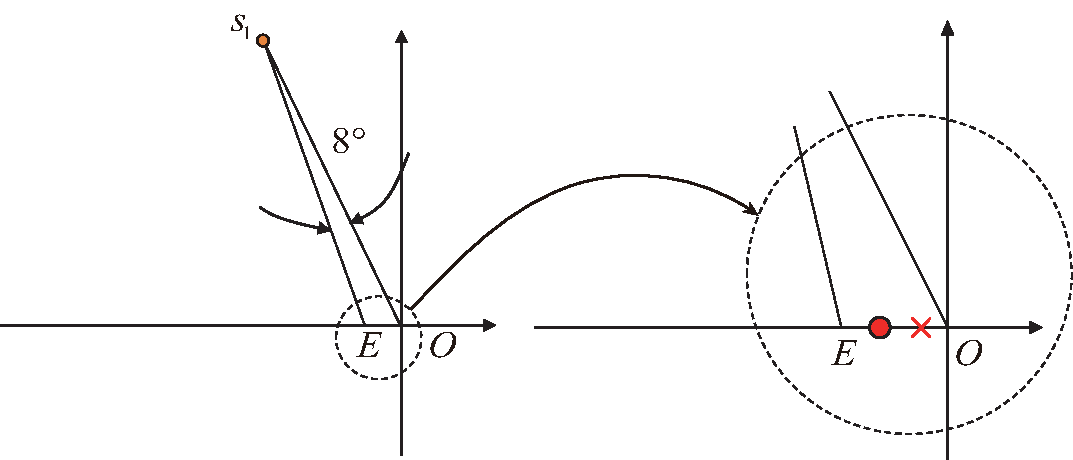
\includegraphics[width=0.7\linewidth]{pic/根轨迹滞后.pdf}
		\vspace*{-1em}
		\caption{利用加角线法确定零点和极点的位置}
		\label{根轨迹滞后}
	\end{figure}

	进而,在$E$点的右侧选择零点和极点.
	\item \textbf{计算校正后系统的期望主导极点并确定补偿器开环增益$\bm{K_\text{c}^*}$的值}\\
	由于动态性能指标不变,利用给定的阻尼比$\zeta$并利用待定系数法确定主导极点及$K_\text{c}^*$的值。
\end{enumerate}

\examples \label{6.5} 已知单位负反馈系统的开环传递函数为
\[
G(s) = \dfrac{1.06}{s(s+1)(s+2)}
\]
设计一个校正器,使得其阻尼比为$\zeta = 0.5$,静态速度误差$e_{\text{ss}} = 0.2.$

\solve 由上述方法解题
\begin{enumerate}[\textbf{第} 1 \textbf{步}]
	\item \textbf{绘制原系统的根轨迹,并根据动态性能指标确定期望的闭环主导极点在复平面上的位置}\\
	由系统的闭环特征方程
	\[
	s(s+1)(s+2)+1.06 = 0
	\]
	可以解得系统的主导极点为
	\[
	s_{1,2} = -0.33 \pm \j 0.59
	\]
	\item \textbf{确定校正器的类型}\\
	其中,$s_{1,2}$与$60 \degree$线接近,而$K_\text{v} = \dfrac{1.06}{2} = 0.53 \le 5$,所以动态性能很好但是不满足静态误差,需要滞后校正器。设滞后校正器为
	\[
	G_{\text{c}}(s) = K_\text{c}^* \dfrac{s - z}{s - p}
	\]
	\item \textbf{求满足指标的稳态误差系数并确定补偿器需要增加的开环增益}\\
	\[
	K_\text{v}^* = \dfrac{1}{e_{\text{ss}}} = \dfrac{1}{0.2} = 5, \quad \Rightarrow \quad K^* = \dfrac{K_\text{v}^*}{K_\text{v}} \approx 10.
	\]
	\item \textbf{利用加角线法确定零点和极点的位置}\\
	过$s_1$作一条直线,与原点$O$和$s_1$间的夹角为$6\degree \sim 10\degree$ 且与横轴交于$E$点,如图\ref{6.5.2}.
	\begin{figure}[!htb]
		\centering
		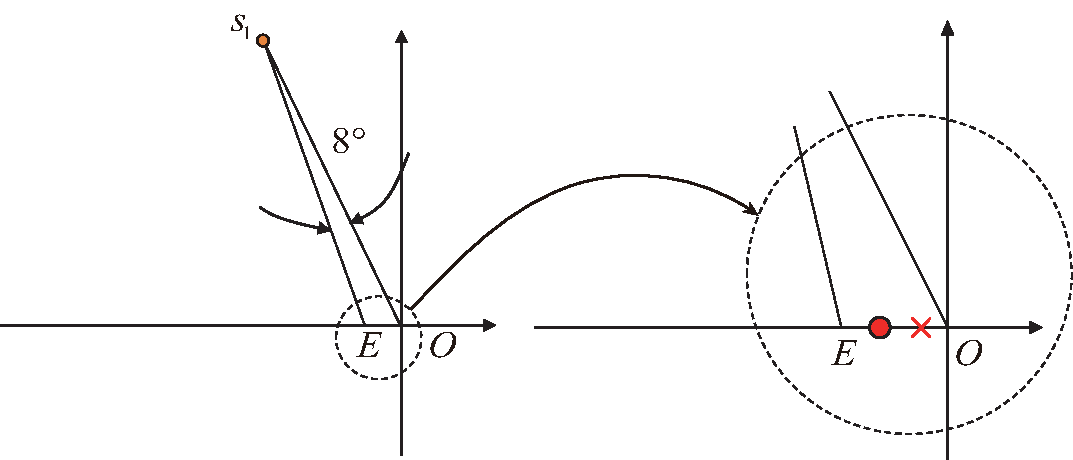
\includegraphics[width=0.7\linewidth]{pic/根轨迹滞后.pdf}
		\vspace*{-1em}
		\caption{\ref{6.5}$\,$确定零点和极点的位置}
		\label{6.5.2}
	\end{figure}

	进而,在$E$点的右侧选择零点和极点:
	\[
	z = -0.05, \quad p = -0.005
	\]
	则校正后的系统为
	\[
	G'(s) = K_c^* \dfrac{s + 0.05}{s + 0.005} \dfrac{1.06}{s(s+1)(s+2)} = K^* \dfrac{s + 0.05}{s(s+1)(s+2)(s+0.005)}
	\]
	\item \textbf{计算校正后系统的期望主导极点并确定补偿器开环增益$\bm{K_\text{c}^*}$的值}\\
	闭环特征方程为
	\begin{align*}
		& \quad \, s(s+1)(s+2)(s+0.005) + K^*s(s+0.05) \\&= s^4 + \dfrac{601}{200}s^3 + \dfrac{403}{200}s^2 + \dfrac{200K^*+2}{200}s + \dfrac{10}{200}K^*\\
		& = (s^2 +2\zeta \omega_\n s + \omega_{\n}^2)(s + s_3)(s + s_4)
	\end{align*}
	
	
	
	
\end{enumerate}
所以校正器和校正后的系统方程分别为
\begin{align*}
	G_\text{c} (s) &=4.68 \dfrac{s + 2.93}{s + 5.46}\\[0.5em]
	G'(s) &= 18.7 \dfrac{4(s + 2.93)}{s(s+2)(s+5.46)}
\end{align*}




\section{反馈校正}
\begin{figure}[!htb]
	\centering
	\begin{tikzpicture}[circuit ee IEC,node distance=1.2cm]
		\node[bulb] (A) [draw, inner sep = 5pt, label=-85:$-$]{};
		\node (A1) [draw, inner sep = 6pt, right of  = A, node distance = 1.5cm]{$G_1(s)$};
		\node[bulb] (B) [draw, right of = A1, node distance = 1.5cm,inner sep = 5pt, label=-85:$-$]{};
		\node (C) [draw, inner sep =6pt, right of = B,node distance =1.5cm]{$G_2(s)$};
		\node (C1) [draw, inner sep =6pt, below of = C,node distance =1.5cm]{$H(s)$};
		\node (D) [draw, inner sep =6pt, right of = C,node distance = 2.5cm]{$G_3(s)$};
		
		\draw[arrows={-Stealth}] (-1.2cm, 0cm) -- (A)node[near start, above = 0cm]{$R(s)$};
		\draw[arrows={-Stealth}] (A) -- (A1);
		\draw[arrows={-Stealth}] (A1) -- (B);
		\draw[arrows={-Stealth}] (B) -- (C);
		\draw[arrows={-Stealth}] (C) -- (D);
		\draw[arrows={-Stealth}] (D) -- +(2cm, 0cm)node[near end, above = 0cm]{$C(s)$};
		\draw [arrows={-Stealth}] (5.7cm, 0cm) -- +(0cm, -1.5cm) -- (C1);
		\draw [arrows={-Stealth}] (C1) -- +(-1.5cm, 0cm) -- (B);
		\draw [arrows={-Stealth}] (8.3cm, 0cm) -- +(0cm, -2.3cm) -- (0cm, -2.3cm) -- (A);
		
	\end{tikzpicture}
	\caption{反馈校正系统结构图}
	\label{反馈校正系统结构图}
\end{figure}

引进$H(s)$的作用是希望$\varPhi_2(s)$的特性使整个闭环系统的品质得到改善。

\subsection{利用反馈改变局部结构、参数}
如图\ref{反馈校正系统结构图}.通过反馈校正可以改变局部结构和参数。
\vspace*{1em}

\noindent \textbf{1. 用位置反馈包围积分环节}
\begin{align}
	G_2(s) = \dfrac{K}{s}
\end{align}
引入反馈
\begin{align}
	H(s) = K_f
\end{align}
得到
\begin{equation}
	\varPhi_2(s) = \dfrac{1}{K_f} \cdot \dfrac{1}{Ts + 1}, \quad T = \dfrac{1}{KK_f}
\end{equation}
所以反馈校正后的结果为
\begin{itemize}
	\item 积分环节变成一阶系统,使系统的无差度下降
	\item 若$T \downarrow$,相位滞后减少,可提高系统的稳定性
\end{itemize}
\vspace*{1.5em}


\noindent \textbf{2.用速度反馈包围惯性、积分和放大环节}
\begin{align}
	G_2(s) = \dfrac{K}{s(Ts + 1)}
\end{align}
引入速度反馈
\begin{align}
	H(s) = K_t s
\end{align}
得到
\begin{align}
	\varPhi_2(s) = \dfrac{K_1}{(Ts + 1)}
\end{align}
所以反馈校正后的结果为
\begin{itemize}
	\item 没有改变典型环节的类型,保持了积分环节,系统的无差度无改变
	\item 因$K_t>0 \rightarrow T_1<T$,可增大系统频宽,有利于加快系统响应
\end{itemize}
\vspace*{1.5em}

\noindent \textbf{3. 用速度反馈包围一个小阻尼的二阶振荡环节和放大环节}
\begin{align}
	G(s) = \dfrac{K \omega_\n^2}{s^2 + 2\zeta \omega_\n s + \omega_{\n}^2 }, \quad 0< \zeta < 1
\end{align}
引入速度反馈
\begin{align}
	H(s) = K_t s
\end{align}
得到
\begin{align}
	\varPhi_2(s) = \dfrac{K\omega_\n^2}{s^2 + 2 \left(\zeta + 0.5 KK_t \omega_\n \right) \omega_\n s+ \omega_\n^2}
\end{align}
所以反馈校正后的结果为:加入速度反馈,增加了阻尼,减弱了小阻尼环节的不利影响。

\noindent \textbf{4. 速度反馈信号再经过一个微分网络}
\begin{align}
	G_2(s) = \dfrac{K_1}{(T_1 s + 1)}
\end{align}
速度反馈信号再经过一个微分网络
\begin{align}
	H(s) = K_t s \dfrac{T_2 s}{T_2 s + 1} = \dfrac{K_t T_2 s^2}{T_2s + 1}
\end{align}
\begin{align}
	\varPhi_2(s) &= \dfrac{K_1(T_2 s + 1)}{s \left[T_1T_2s^2 + \left(T_1 + T_2 + T_2K_1K_t\right)s + 1 \right]}\notag \\[0.5em]
	& =\dfrac{K_1(T_2s + 1)}{s(T's + 1)(T''s + 1)} =\dfrac{K_1(T_1s + 1)(T_2s + 1)}{s(T_1s + 1)(T's + 1)(T''s + 1)}\\
	T' + T'' &= T_1 + T_2 + K_1K_tT_2\notag \\
	T'T'' &= T_1 T_2\notag
\end{align}

\subsection{利用反馈削弱非线性因素的影响}
最典型的例子是高增益的运算放大器。由
\begin{equation}
	\varPhi(\j \omega) = \dfrac{G(\j \omega)}{1 + G(\j \omega) H(\j \omega)}
\end{equation}
若满足
\begin{equation}
	|G(\j \omega)H(\j \omega) >> 1|
\end{equation}
则
\begin{equation}
	\varPhi(\j \omega) = \dfrac{G(\j \omega)}{1 + G(\j \omega)H(\j \omega)} \approx \dfrac{1}{H(\j \omega)}
\end{equation}
说明$\varPhi(\j \omega)$主要取决于$H(\j \omega)$,而与$G(\j \omega)$无关。

若反馈元件的线性度比较好,特性比较稳定,
那么反馈结构的线性度也好,特性也比较稳定,
正向回路中非线性因素、元件参数不稳定等不
利因素均可以削弱。
\vspace*{1em}

\subsection{反馈可提高模型摄动的不灵敏性}
\vspace*{-1em}
\begin{figure}[!htb]
	\centering
	\subfigure[串联校正]{
		\begin{minipage}{0.45\linewidth}
			\centering
			\begin{tikzpicture}[circuit ee IEC]
				%定义流程图具体形状
				\node[bulb] (A) [inner sep = 5pt, draw, label = -95:$-$]{};
				\node (B) [inner sep = 5pt, right of = A, node distance = 1.5cm, draw]{$K_{\text{c}}(s)$};
				\node (C) [inner sep = 5pt, right of = B, node distance = 1.7cm, draw]{$G(s)$};
				
				%连接具体形状
				\draw[arrows={-Stealth}](-1cm, 0cm) -- (A)node[near start, above = 0cm]{$X_1$};
				
				\draw[arrows={-Stealth}](A) -- (B) ;
				\draw[arrows={-Stealth}](B) -- (C) ;
				\draw[arrows={-Stealth}](C) -- +(1.5cm,0)node[very near end, above = 0cm]{$X_0$} ;
				\draw[arrows={-Stealth}](4.3cm , 0cm) -- (4.3cm, -1.2cm) -- (0cm,-1.2cm) -- (A) ;
			\end{tikzpicture}
		\label{串联不灵敏}
		\vspace*{1.8em}
		\end{minipage}
}
	\subfigure[反馈校正]{
	\begin{minipage}{0.45\linewidth}
		\centering
		\begin{tikzpicture}[circuit ee IEC]
			%定义流程图具体形状
			\node[bulb] (A) [inner sep = 5pt, draw, label = -95:$-$]{};
			\node (B) [inner sep = 5pt, right of = A, node distance = 1.5cm, draw]{$K_{\text{c}}(s)$};
			\node (C) [inner sep = 5pt, below of = B, node distance = 1.2cm, draw]{$H(s)$};
			
			%连接具体形状
			\draw[arrows={-Stealth}](-1cm, 0cm) -- (A)node[near start, above = 0cm]{$X_1$};
			
			\draw[arrows={-Stealth}](A) -- (B) ;
			\draw[arrows={-Stealth}](B) -- +(2cm,0)node[very near end, above = 0cm]{$X_\text{c}$} ; 
			\draw[arrows={-Stealth}](3cm , 0cm) --+(0cm, -1.2cm) -- (C);
			\draw[arrows={-Stealth}](C) -- (0cm,-1.2cm) -- (A) ;
		\end{tikzpicture}
	\vspace*{1em}
	\label{反馈不灵敏}
	\end{minipage}
}
	\vspace*{-0.5em}
	\caption{系统的串联校正和反馈校正}
	\label{校正的不灵敏性}
\end{figure}

\begin{itemize}
	\item 摄动是由于模型参数变化或某些不确定因素引起的
	\item 采取反馈校正比串联校正对模型的摄动更为不敏感
\end{itemize}

如图\ref{校正的不灵敏性},当$K_\text{c}(s) = \dfrac{1}{1+G(s)H(s)}$的时候,$X_0 = X_c$,当$G(s)$参数变化变成$G^*(s)$的时候,两种方式的输出稳态误差分别为
\begin{align}
	E_\text{c}(s) = \left(\dfrac{G(s)}{1 + G(s)H(s)} - \dfrac{G^*(s)}{1+G^*(s)H(s)} \right)X_1\\[0.5em]
	E_0(s) = \left(\dfrac{G(s)}{1+G(s)H(s)}- \dfrac{G^*(s)}{1+G(s)H(s)}\right)X_1
\end{align}
所以,
\begin{equation}
	\dfrac{E_\text{c}(s)}{E_0(s)} = \dfrac{1}{1+G^*(s)H(s)}
\end{equation}

\noindent 进而得到$\big|1 + G^*(s)H(s)\big|>1 \quad \Rightarrow \quad \big|E_\text{c}(s)\big| < \big|E_0(s)\big|$,一般来说做到这个是不困难(很常见)的。
\vspace*{1em}

\subsection{利用反馈抑制干扰}
\begin{figure}[!htb]
	\centering
	\begin{tikzpicture}[circuit ee IEC]
		%定义流程图具体形状
		\node[bulb] (A) [inner sep = 5pt, draw, label = -95:$-$]{};
		\node (B) [inner sep = 5pt, right of = A, node distance = 1.5cm, draw]{$K_{\text{c}}(s)$};
		\node[bulb] (D) [inner sep = 5pt, draw, label = -95:$-$, right of = B, node distance = 1.5cm]{};
		\node (C) [inner sep = 5pt, below of = B, node distance = 2cm, draw]{$H(s)$};
		\node[bulb] (E) [inner sep = 5pt, draw, below of = A, xshift = 4cm,  node distance = 1cm]{};
		
		%连接具体形状
		\draw[arrows={-Stealth}](-1cm, 0cm) -- (A)node[near start, above = 0cm]{$R=0$};
		
		\draw[arrows={-Stealth}](A) -- (B) ;
		\draw[arrows={-Stealth}](D) -- +(1.5cm,0)node[very near end, above = 0cm]{$X_\text{c}$} ; 
		\draw[arrows={-Stealth}](4cm , 0cm) --(E) --+(0cm, -1cm) -- (C);
		\draw[arrows={-Stealth}](C) -- (0cm,-2cm) -- (A) ;
		\draw[arrows={-Stealth}] (B) -- (D);
		
		\draw[arrows={-Stealth}] (3cm, 1cm) -- (D)node[near start, above = 0.1cm]{$N(s)$};
		\draw[arrows={-Stealth}] (5cm, -1cm) -- (E)node[near start, above = 0cm]{$\eta$};
	\end{tikzpicture}
	\caption{利用反馈抑制干扰}
\end{figure}
干扰传递函数为
\begin{align}
	X_\text{c}(s) = \dfrac{1}{1+G(s)H(s)}N(s)
\end{align}

可以看出,只要$\big|1+G(s)H(s)\big| > 1$,干扰$N$的影响就可以得到抑制。但引入反馈$H(s)$会产生测量噪声$\eta$,从抑制$\eta$的角度,其传递函数为
\begin{align}
	X_\text{c}(s) = \dfrac{G(s)H(s)}{1+G(s)H(s)}\eta
\end{align}

可以看出,其要求高频区$\big|G(s)H(s)\big| << 1$。一般来说,若$\eta$发生在高频段,在高频段满足$\big|G(s)H(s)\big| << 1$和低频段$\big|G(s)H(s)\big| >> 1$并不矛盾。


\section{复合校正}
对于稳态精度、平稳性和快速性要求都很高的系统,或对受到经常作用的强干扰的系统,除了在主反馈回路内部进行串联校正或局部反馈校正外,往往还同时采取设置在回路之外的前置校正或干扰补偿校正。这种开式、闭式相结合的校正,称为\dy[复合校正]{FHJZ}。具有复合校正的控制系统称为\dy[复合控制系统]{FHKZXT}。
\vspace*{1em}

\subsection{对控制作用对附加前置校正}
\begin{figure}[!htb]
	\centering
	\begin{tikzpicture}[circuit ee IEC]
		%定义流程图具体形状
		\node[bulb] (A) [inner sep = 5pt, draw, label = -95:$-$]{};
		\node (A1) [inner sep = 6pt, draw, above of = A, node distance = 1.5cm]{$\,\, G_\text{c}(s) \,\,$};
		\node[bulb] (B) [inner sep = 5pt, draw, right of = A, node distance = 1.5cm]{};
		\node (B1) [inner sep = 6pt, draw, right of = B, node distance = 1.5cm]{$\,\, G(s) \,\,$};
		
		%连接具体形状
		\draw[arrows={-Stealth}](-2.8cm, 0cm) -- (A)node[very near start, above = 0cm]{$R(s)$};
		\draw[arrows={-Stealth}](A) -- (B)node[midway, above = 0cm]{$E(s)$};
		\draw[arrows={-Stealth}](B) -- (B1);
		\draw[arrows={-Stealth}](B1) --+ (2cm, 0cm)node[near end, above = 0cm]{$C(s)$};
		\draw[arrows={-Stealth}](-1.5cm,0cm) -- +(0cm, 1.5cm) -- (A1);
		\draw[arrows={-Stealth}](A1) --+ (1.5cm, 0cm) -- (B);
		\draw[arrows={-Stealth}](4cm, 0cm) --+(0cm, -1.5cm) -- (0cm, -1.5cm) -- (A);
	\end{tikzpicture}
	\caption{对控制作用对附加前置校正}
	\label{对控制作用对附加前置校正}
\end{figure}

如图\ref{对控制作用对附加前置校正},系统闭环传递函数
\begin{align}
	\dfrac{C(s)}{R(s)} = \big[1 + G_\text{c}(s)\big]\dfrac{G(s)}{1+G(s)}
\end{align}
希望系统输出完全复现控制输入,即
\begin{equation}
	E(s) = R(s) - C(s) = \left(1 - \dfrac{C(s)}{R(s)}\right)R(s) = \dfrac{1 - G(s)G_\text{c}(s)}{1 + G(s)} R(s) = 0
\end{equation}
最简单的构造方法是
\begin{equation}
	G_\text{c}(s) = G^{-1}(s)
\end{equation}
但这在物理上有时难以实现,特别是当$G(s)$具有右半平面零点时。因此,需要采用其它补偿方法。

设
\begin{align}
	G(s) = \dfrac{N(s)}{D(s)} &= \dfrac{b_ms^m + \cdots + b_1s + b_0}{s^n + a_{n-1}s^{n-1} + \cdots + a_1 s + a_0}, \quad m \le n\\
	G_\text{c}(s) &= d_2s^2 + d_1s^1+d_0
\end{align}
此时误差函数为
\begin{equation}
	\dfrac{E(s)}{R(s)} = \dfrac{1 -G_\text{c}(s)G(s)}{1+G(s)} = \dfrac{s^n + a_{n-1}s^{n-1} + \cdots + a_1s + a_0 - \big(d_2 s^2 + d_1 s^1 + d_0\big)\big(b_ms^m + \cdots + b_1 s + b_0\big)}{s^n + \cdots + (a_m+b_m)s^m + \cdots (a_0 + b_0)}
\end{equation}

取$s^2,s^1,s^0$的系数
\begin{align}
	s^0& \quad a_0-d_0b_0 \label{s0} \\
	s^1 &\quad a_1 - (d_1b_0+d_0b_1) \label{s1} \\
	s^2 &\quad a_2 - (b_2d_0+b_1d_1+b_0d_2) \label{s2}
\end{align}
则可以得到一下结论
\begin{enumerate}[\hspace*{2em} 1. ]
	\item 误差函数存在1个$s$因子 \quad$\rightarrow$ \quad  系统的无差度为1 \quad$\rightarrow$ \quad \eqref{s0}$\,\, = 0.$
	\item 误差函数存在2个$s$因子 \quad$\rightarrow$ \quad 系统的无差度为2 \quad$\rightarrow$ \quad \eqref{s0}, \eqref{s1}$\,\, = 0$
	\item 误差函数存在3个$s$因子 \quad$\rightarrow$ \quad 系统的无差度为3 \quad$\rightarrow$ \quad \eqref{s0}, \eqref{s1}, \eqref{s2}$\,\, = 0$
\end{enumerate}

\examples \label{6.6}已知系统的结构图如图\ref{F6.6}.
\begin{figure}[!htb]
	\centering
	\begin{tikzpicture}[circuit ee IEC]
		%定义流程图具体形状
		\node[bulb] (A) [inner sep = 5pt, draw, label = -95:$-$]{};
		\node (A1) [inner sep = 6pt, draw, above of = A, node distance = 1.5cm]{$\,\, G_\text{c}(s) \,\,$};
		\node[bulb] (B) [inner sep = 5pt, draw, right of = A, node distance = 1.5cm]{};
		\node (B1) [inner sep = 6pt, draw, right of = B, node distance = 3cm]{$\,\, \dfrac{0.855}{s(0.1s+1)(0.05s+1)} \,\,$};
		
		%连接具体形状
		\draw[arrows={-Stealth}](-2.8cm, 0cm) -- (A)node[very near start, above = 0cm]{$R(s)$};
		\draw[arrows={-Stealth}](A) -- (B)node[midway, above = 0cm]{$E(s)$};
		\draw[arrows={-Stealth}](B) -- (B1);
		\draw[arrows={-Stealth}](B1) --+ (3cm, 0cm)node[near end, above = 0cm]{$C(s)$};
		\draw[arrows={-Stealth}](-1.5cm,0cm) -- +(0cm, 1.5cm) -- (A1);
		\draw[arrows={-Stealth}](A1) --+ (1.5cm, 0cm) -- (B);
		\draw[arrows={-Stealth}](7cm, 0cm) --+(0cm, -1.5cm) -- (0cm, -1.5cm) -- (A);
	\end{tikzpicture}
	\caption{\ref{6.6}$\,$的系统结构图}
	\label{F6.6}
\end{figure}

\noindent 设计一尽可能简单的$G_\text{c}(s)$,使得当$r(t)=t·1(t)$时无稳态误差。

\solve 由梅森公式及误差函数的定义,
\begin{align*}
	E(s) &= C(s) - R(s) = \dfrac{1-G(s)G_{\text{c}(s)}}{1+G(s)} R(s)\\[0.5em]
	& = \dfrac{s(0.1s+1)(0.05s+1) - 0.855G_{\text{c}}(s)}{s(0.1s+1)(0.05s+1)+0.855} \times \dfrac{1}{s^2}
\end{align*}
由劳斯定理可判定系统稳定,利用终值定理,
\begin{align*}
	e_{\text{ss}} &= \lim\limits_{s\to 0} sE(s)\\[0.5em]
	& = \dfrac{s(0.1s+1)(0.05s+1) - 0.855G_{\text{c}}(s)}{s(0.1s+1)(0.05s+1)+0.855} \times \dfrac{1}{s}
\end{align*}
令
\begin{equation*}
	0.855G_{\text{c}}(s) = s \quad \Rightarrow \quad G_{\text{c}}(s) = \dfrac{s}{0.855}
\end{equation*}
则
\begin{align*}
	e_{\text{ss}} & = \lim\limits_{s \to 0} \dfrac{0.005s^3+0.01s^2}{s(0.1s+1)(0.05s+1)+0.855} \times \dfrac{1}{s} \\[0.5em]
	& = \lim\limits_{s \to 0} \dfrac{0.005s^2+0.01s}{s(0.1s+1)(0.05s+1)+0.855} = 0
\end{align*}
\vspace*{-3em}
\warn[
{
	\begin{enumerate}[\hspace*{1em} 1. ]
		\item 需要讨论系统的稳定性。\vspace*{-0.5em}
		\item 使用终值定理的条件是$sE(s)$的根的实部小于0.
	\end{enumerate}
}
]


\subsection{对干扰的附加补偿校正}
对于扰的补偿控制也是一种前置校正方式
\begin{figure}[!htb]
	\centering
	\begin{tikzpicture}[circuit ee IEC]
		\node(A) [draw, inner sep =6pt]{$G_1(s)$};
		\node[bulb] (C) [draw, inner sep = 5pt, right of = A, node distance = 1.5cm, label = 95:$+$] {};
		\node (D) [draw, inner sep = 6pt, right of = C, node distance = 1.5cm]{$G_2(s)$};
		\node[bulb] (O) [draw, inner sep =5pt, left of = A, node distance = 1.7cm, label = -95:$-$]{};
		\node (B) [draw, inner sep =6pt, above of = A, node distance = 1.5cm]{$G_\text{c}(s)$};
		
		\draw[arrows={-Stealth}](-3cm, 0) -- (O)node[near start, above = 0mm]{$R(s)$};
		\draw[arrows={-Stealth}](O) -- (A);
		\draw[arrows={-Stealth}](A)-- (C);
		\draw[arrows={-Stealth}](C) -- (D);
		\draw[arrows={-Stealth}](D) -- +(1.5cm, 0cm)node[midway, above = 0mm,xshift = 5mm]{$C(s)$};
		\draw[arrows={-Stealth}](4cm, 0cm) -- +(0cm, -1.2cm)  -- (-1.7cm,-1.2cm) -- (O);
		\draw[arrows={-Stealth}](1.5cm, 2.5cm) -- (C)node[near start, xshift = 0.5cm]{$N(s)$};
		\draw[arrows={-Stealth}, dashed](1.5cm, 1.5cm) -- (B);
		 \draw[arrows={-Stealth}, dashed] (B) --+ (-1.7cm, 0cm) -- (O);
	\end{tikzpicture}
	\caption{干扰的前置补偿1}
	\label{干扰的前置补偿}
\end{figure}

干扰对系统的传递函数为
\begin{equation}
	\dfrac{C(s)}{N(s)} = \dfrac{G_2(s)\big[1 + G_1(s)G_\text{c}(s)\big]}{1 + G_1(s)G_2(s)}
\end{equation}
为了使干扰不影响系统,使传递函数为0,即
\begin{equation}
	G_\text{c}(s) = \dfrac{1}{G_1(s)}
\end{equation}
方法特点
\begin{itemize}
	\item 单纯依靠回路的设计来达到抑制干扰,有一定的困难与不便。\vspace*{-0.5em}
	\item 利用附加的干扰补偿装置,实现干扰对系统输出的不变性,是一种非常有效的方法。
\end{itemize}

\textbf{另一种干扰的补偿控制方式如图\ref{干扰的前置补偿2}.}
\begin{figure}[!htb]
	\centering
	\begin{tikzpicture}[circuit ee IEC]
		\node(A) [draw, inner sep =6pt]{$G_1$};
		\node (B) [draw, inner sep =6pt, above of = A, node distance = 2.5cm]{$W_1$};
		\node[bulb] (C) [draw, inner sep = 5pt, right of = A, node distance = 1.5cm] {};
		\node (D) [draw, inner sep = 6pt, right of = C, node distance = 1.5cm]{$G_2$};
		\node[bulb] (O) [draw, inner sep =5pt, left of = A, node distance = 1.7cm, label = -95:$-$]{};
		\node[bulb] (E) [draw, inner sep = 5pt, right of = D, node distance = 1.5cm] {};
		\node[bulb] (F) [draw, inner sep = 5pt, above of = C, node distance = 2.5cm,label = 5:$-$,label = 175:$+$,label = -85:$x$] {};
		\node (G) [draw, inner sep =6pt, above of = D, node distance = 2.5cm]{$W_2$};
		\node (H) [draw, inner sep =6pt, above of = C, node distance = 1.25cm]{$W_3$};
		
		\draw[arrows={-Stealth}](-3.5cm, 0) -- (O)node[near start, above = 0mm]{$R(s)$};
		\draw[arrows={-Stealth}] (O) -- (A);
		\draw[arrows={-Stealth}] (A) -- (C);
		\draw[arrows={-Stealth}] (C) -- (D);
		\draw[arrows={-Stealth}] (D) -- (E);
		\draw[arrows={-Stealth}] (E) -- +(2cm,0cm)node[near end, above = 0cm]{$C(s)$};
		\draw[arrows={-Stealth}] (5.5cm, 0cm) --+ (0cm, 2.5cm) -- (G);
		\draw[arrows={-Stealth}] (-2.5cm,0cm) --+ (0cm, 2.5cm) -- (B);
		\draw[arrows={-Stealth}] (B) -- (F);
		\draw[arrows={-Stealth}] (G) -- (F);
		\draw[arrows={-Stealth}] (F) -- (H);
		\draw[arrows={-Stealth}] (H) -- (C);
		\draw[arrows={-Stealth}] (5.5cm, 0cm) --+ (0cm, -1.5cm) -- (-1.7cm, -1.5cm) -- (O);
		\draw[arrows={-Stealth}]  (4.5cm,1.25cm) -- (E)node[near start, xshift = -5mm, yshift =1mm]{$N(s)$};
		
	\end{tikzpicture}
	\vspace*{-0.5em}
	\caption{干扰的前置补偿2}
	\label{干扰的前置补偿2}
\end{figure}

在未加补偿之前,系统的输出函数为
\begin{equation}
	C(s) = \dfrac{G_1G_2}{1+G_1G_2}R(s) + \dfrac{1}{G_1G_2}N(s)
\end{equation}
在加上补偿后,系统的输出为
\begin{equation}
	C(s) = \dfrac{G_2(G_1+W_1W_3)}{1+G_2(G_1+W_2W_3)}R(s) + \dfrac{1}{1 + G_2(G_1+W_2W_3)}N(s)
\end{equation}
若$N(s) = 0$且使
\begin{equation}
	W_1 = \dfrac{G_1G_2}{1+G_1G_2}, \quad W_2 = 1
\end{equation}
则此时
\begin{equation}
	C(s)= \dfrac{G_1G_2}{1+G_1G_2}R(s)
\end{equation}

这说明当没有干扰时,结构图表示的关系可以保持输入与输出的关系不变。这时附加部分的输出相抵消,此时图\ref{干扰的前置补偿2}中的信号$x = 0.$
\vspace*{0.5em}

当$N(s) \neq 0$时,若增益$\big|W_3\big|$很大,且仍满足
\begin{equation*}
	W_1 = \dfrac{G_1G_2}{1+G_1G_2}, \quad W_2 = 1
\end{equation*}
则干扰$N(s)$的影响仍可被抑制。








